\documentclass{beamer}

\usetheme{zg}

\title{RESTful API}
\date{\today}
\author{Fernando Camargo}
\institute{ZG Soluções}


\begin{document}
\maketitle

\section{Por que REST?}

\begin{frame}{Web App vs Web Service}
  \begin{outline}
    \1<1-> Aplicações Web convencionais
  \0 \visible<1->{\resizebox{!}{1in}{\includesvg{Web-Applications}}}
    \1<2-> Web Services
  \0 \visible<2->{\resizebox{!}{1in}{\includesvg{Web-Services}}}
  \end{outline}
\end{frame}

\begin{frame}{Menor gasto de rede}
  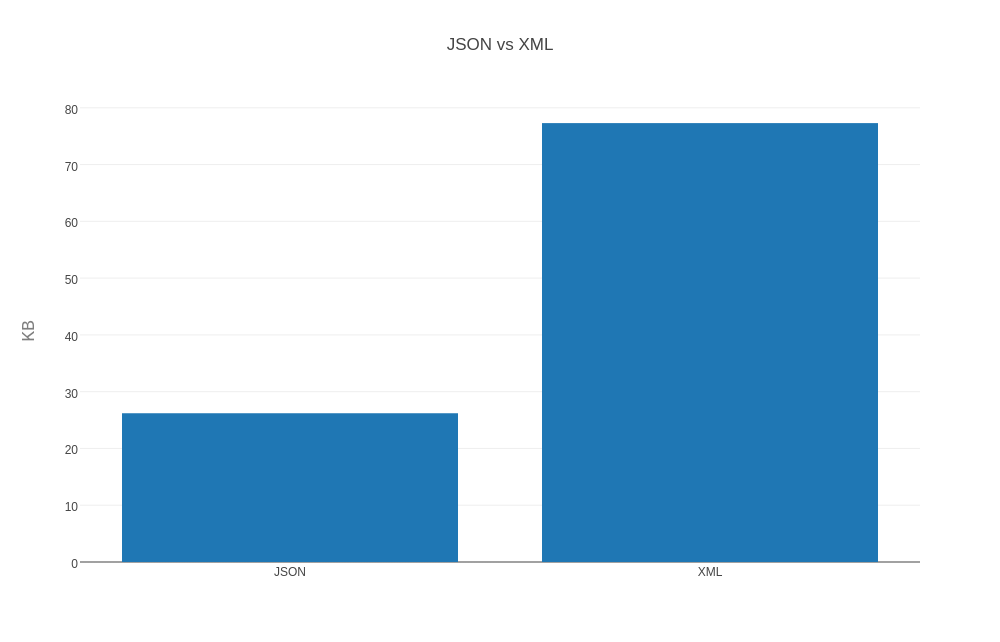
\includegraphics[width=\textwidth]{JSON-vs-XML}\\
  {\tiny Fonte: \cite{davelaar2015}}
\end{frame}

\begin{frame}{Melhor performance}
  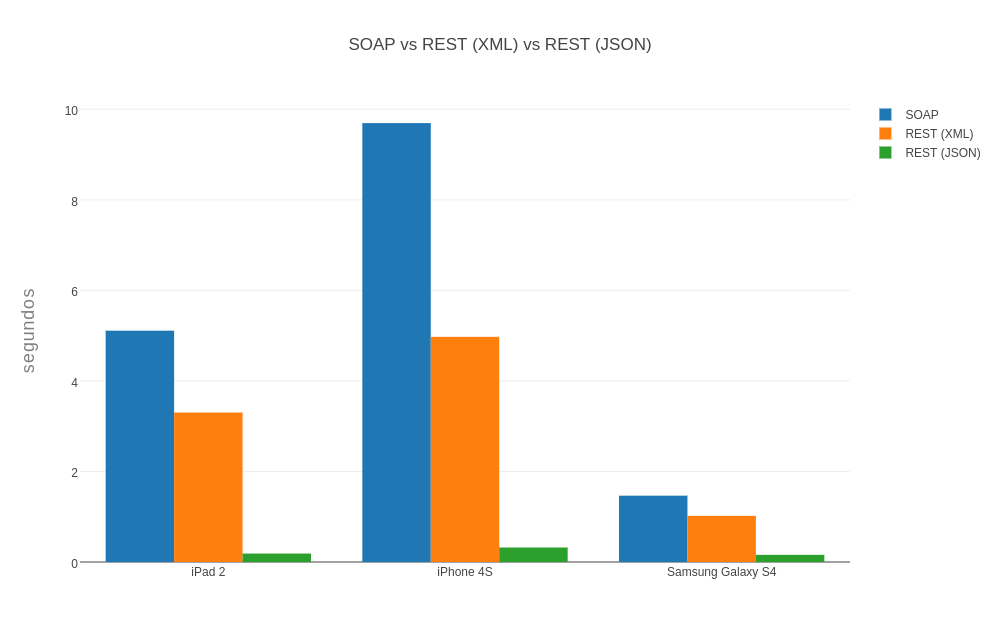
\includegraphics[width=\textwidth]{SOAP-vs-REST}\\
  {\tiny Fonte: \cite{davelaar2015}}
\end{frame}


\begin{frame}{SOAP vs REST}
  \begin{table}[]
    \begin{tabular}{@{}ll@{}}
      \toprule
      \textbf{SOAP}                       & \textbf{REST}                           \\ \midrule
      Especificação                       & Padrão arquitetural                     \\ \pause
      Projetado para \alert{servidores}   & Projetado para \alert{clientes leves}   \\ \pause
      Stateful                            & Stateless                               \\ \pause
					  & Possibilita cache                       \\ \pause
      Baseado em ações                    & Baseado em recursos                     \\ \bottomrule
    \end{tabular}
  \end{table}
\end{frame}

\section{Padrão Arquitetural do REST}

\begin{frame}{Regras}
  \begin{outline}
    \1<1-> Inferface Uniforme
    \1<2-> Stateless
    \1<3-> Cacheable
    \1<4-> Cliente-Servidor
      \2 Servidor: armazenamento de dados
      \2 Cliente: apresentação e manutenção de sessão
    \1<5-> Sistema em Camadas (possibilidade)
    \1<6-> Código sob Demanda (possibilidade)
  \end{outline}
\end{frame}

\subsection{Inferface Uniforme}

\begin{frame}{Interface Uniforme}
  \begin{outline}
    \1<1-> Baseada em \alert{recursos}
    \1<2-> Recursos identificados por URL
    \1<3-> Ações por métodos HTTP
    \1<4-> URLs com substantivos no plural
  \end{outline}
\end{frame}

\begin{frame}{URLs Incorretas}
  \begin{outline}
    \1 /listarProdutos
    \1 /obterProdutos/1
    \1 /criarProdutos
    \1 /deletarProdutos/1
  \end{outline}
\end{frame}

\begin{frame}{URLs Corretas}
  \begin{outline}
    \1 /produtos
    \1 /produtos/1
  \end{outline}
\end{frame}

\begin{frame}{Interface Uniforme}
  \begin{outline}
    \1<1-> \textbf{Re}presentational \textbf{S}tate \textbf{T}ransfer
    \1<2-> \textbf{HATEOAS}: \textbf{H}ypermedia \textbf{a}s \textbf{t}he \textbf{E}ngine \textbf{o}f \textbf{A}pplication \textbf{S}tate 
    \1<3-> Mensagens autodescritivas
  \end{outline}
\end{frame}

\subsection{Protocolo HTTP}

\begin{frame}{Métodos HTTP}
  \begin{table}[]
  \begin{tabular}{@{}lll@{}}
  \toprule
  Método & Ação                                   & Idempotente \\ \midrule
  GET    & Obtenção                               & Sim         \\ \pause
  HEAD   & Obtenção de metadados                  & Sim         \\ \pause
  DELETE & Remoção                                & Sim         \\ \pause
  POST   & Criação sem ID ou atualização parcial  & Não         \\ \pause
  PUT    & Criação com ID ou atualização completa & Sim         \\ \bottomrule
  \end{tabular}
  \end{table}
  {\tiny Idempotência: múltiplas requisições não alteram o resultado}
\end{frame}

\begin{frame}{Status HTTP}
  \begin{outline}
    \1<1-> 200 OK
    \1<2-> 201 Created
    \1<3-> 304 Not Modified
    \1<4-> 400 Bad Request
    \1<5-> 401 Unauthorized
    \1<6-> 403 Forbidden
    \1<7-> 404 Not Found
  \end{outline}
\end{frame}

\section{Boas Práticas}

\subsection{Versionamento}

\begin{frame}{Versionamento}
  \begin{outline}
  \0 Evita quebra de contrato com clientes
    \1<1-> URL
      \2<2-> GET api.zg.com.br/\alert{v1}/guias\\Accept: application/json
      \2<3-> POST api.devmedia.com.br/\alert{v1}/revistas\\Content-Type: application/json\\Body: \mintinline{js}{{"numeroConta": "451618763",...}}
    \1<4-> Media-Type
      \2<5-> GET api.zg.com.br/guias\\Accept: application/\alert{vnd.devmedia.revista-v1}+json
      \2<6-> POST api.zg.com.br/revistas\\Content-Type: application/\alert{vnd.devmedia.revista-v1}+json\\Body: \mintinline{js}{{"numeroConta": "451618763",...}}
  \end{outline}
\end{frame}

\subsection{Representação}

\begin{frame}{Formato de Representação}
  \begin{outline}
    \1<1-> Suportar múltiplos formatos (XML e JSON)
      \2<1-> URL: api.zg.com.br/guias\alert{.json}
      \2<2-> Media-Type (Accept e Content-Type)
    \1<3-> camelCase
    \1<4-> Data e hora: ISO 8601
      \2<4-> UTC
      \2<5-> yyyy-MM-dd'T'HH:mm:ss.SSS'Z' (\alert{2013-09-26}T\alert{21:24:39.521}Z)
  \end{outline}
\end{frame}

\begin{frame}[fragile]{HATEOAS}
  \begin{minted}[fontsize=\tiny,escapeinside=||]{js}
{
  |\alert{\textquotedblright\text{href}\textquotedblright}|: "https://api.zg.com.br/clientes/2g41s",
  "nome": "Fernando Camargo",
  "cpf": "62854828532",
  "idade": 22,
  "telefones": ["6298350912", "6232903845"],
  "email": "fernando.camargo.ti@gmail.com",
  "endereco": {
    |\alert{\textquotedblright\text{href}\textquotedblright}|: "https://api.zg.com.br/enderecos/8502hgo",
    "logradouro": "Rua 12-A",
    "cep": "63905192",
    "bairro": "Setor Aeroporto",
    "numero": 168,
    "complemento": "Apartamento 301",
    "cidade": "Goiânia",
    "estado": "GO",
    "pais": "Brasil"
  }
}
  \end{minted}
\end{frame}

\begin{frame}{Representação Parcial}
  \begin{outline}
    \1<1-> Especificar campos desejados (parâmetro \alert{fields})
    \1<2-> Recursos relacionados
      \2<2-> Trazer apenas \alert{href} por padrão
      \2<3-> Permitir expansão (parâmetro \alert{expand})
  \end{outline}
\end{frame}

\begin{frame}[fragile]{Resposta padrão}
  GET https://api.zg.com.br/clientes/2g41s
  \begin{minted}[fontsize=\tiny,escapeinside=||]{js}
{
  "href": "https://api.zg.com.br/clientes/2g41s",
  "nome": "Fernando Camargo",
  "cpf": "62854828532",
  "idade": 22,
  "telefones": ["6298350912", "6232903845"],
  "email": "fernando.camargo.ti@gmail.com",
  "endereco": {
    |\alert{\textquotedblright\text{href}\textquotedblright}|: "https://api.zg.com.br/enderecos/8502hgo"
  }
}
  \end{minted}
\end{frame}

\begin{frame}[fragile]{Parâmetro \alert{fields}}
  GET https://api.zg.com.br/clientes/2g41s?
  \alert{fields}=nome,cpf,email
  \begin{minted}[fontsize=\tiny,escapeinside=||]{js}
{
  "href": "https://api.zg.com.br/clientes/2g41s",
  "nome": "Fernando Camargo",
  "cpf": "62854828532",
  "email": "fernando.camargo.ti@gmail.com"
}
  \end{minted}
\end{frame}

\begin{frame}[fragile]{Parâmetro \alert{fields}}
  GET https://api.zg.com.br/clientes/2g41s?
  \alert{fields}=nome,cpf,email,endereco
  \begin{minted}[fontsize=\tiny,escapeinside=||]{js}
{
  "href": "https://api.zg.com.br/clientes/2g41s",
  "nome": "Fernando Camargo",
  "cpf": "62854828532",
  "email": "fernando.camargo.ti@gmail.com",
  "endereco": {
    "href": "https://api.zg.com.br/enderecos/8502hgo"
  }
}
  \end{minted}
\end{frame}

\begin{frame}[fragile]{Parâmetro \alert{fields}}
  GET https://api.zg.com.br/clientes/2g41s?
  \alert{fields}=nome,cpf,email,\alert{endereco(cidade,estado,pais)}
  \begin{minted}[fontsize=\tiny,escapeinside=||]{js}
{
  "href": "https://api.zg.com.br/clientes/2g41s",
  "nome": "Fernando Camargo",
  "cpf": "62854828532",
  "email": "fernando.camargo.ti@gmail.com",
  "endereco": {
    "href": "https://api.zg.com.br/enderecos/8502hgo",
    "cidade": "Goiânia",
    "estado": "GO",
    "pais": "Brasil"
  }
}
  \end{minted}
\end{frame}

\begin{frame}[fragile]{Parâmetro \alert{expand}}
  GET https://api.zg.com.br/clientes/2g41s?\alert{expand}=endereco
  \begin{minted}[fontsize=\tiny,escapeinside=||]{js}
{
  "href": "https://api.zg.com.br/clientes/2g41s",
  "nome": "Fernando Camargo",
  "cpf": "62854828532",
  "idade": 22,
  "telefones": ["6298350912", "6232903845"],
  "email": "fernando.camargo.ti@gmail.com",
  "endereco": {
    "href": "https://api.zg.com.br/enderecos/8502hgo",
    "logradouro": "Rua 12-A",
    "cep": "63905192",
    "bairro": "Setor Aeroporto",
    "numero": 168,
    "complemento": "Apartamento 301",
    "cidade": "Goiânia",
    "estado": "GO",
    "pais": "Brasil"
  }
}
  \end{minted}
\end{frame}

\subsection{Paginação}

\begin{frame}{Paginação}
  \begin{outline}
    \1<1-> Parâmetros \alert{offset} e \alert{limit}
    \1<2-> Hyperlinks para paginação
    \1<3-> Possibilidade: trazer apenas \alert{href} por padrão e permitir \alert{expand}
  \end{outline}
\end{frame}

\begin{frame}[fragile]{Resposta Padrão}
  GET https://api.zg.com.br/clientes
  \begin{minted}[fontsize=\tiny,escapeinside=||]{js}
{
  "href": "https://api.zg.com.br/clientes",
  |\alert{\textquotedblright\text{offset}\textquotedblright}|: 0,
  |\alert{\textquotedblright\text{limit}\textquotedblright}|: 10,
  |\alert{\textquotedblright\text{first}\textquotedblright}|: {"href": "https://api.zg.com.br/clientes?offset=0"},
  |\alert{\textquotedblright\text{previous}\textquotedblright}|: null,
  |\alert{\textquotedblright\text{next}\textquotedblright}|: {"href": "https://api.zg.com.br/clientes?offset=10"},
  |\alert{\textquotedblright\text{last}\textquotedblright}|: {"href": "https://api.zg.com.br/clientes?offset=990"},
  "items": [
    {"href": "https://api.zg.com.br/clientes/61h58s"},
    {"href": "https://api.zg.com.br/clientes/f72baf"},
    {"href": "https://api.zg.com.br/clientes/823huf"},
    {"href": "https://api.zg.com.br/clientes/u23hf6"},
    {"href": "https://api.zg.com.br/clientes/fqgy2f"},
    {"href": "https://api.zg.com.br/clientes/vuhq9df"},
    {"href": "https://api.zg.com.br/clientes/vg782qw"},
    {"href": "https://api.zg.com.br/clientes/v90aqga"},
    {"href": "https://api.zg.com.br/clientes/vihaqgt9"},
    {"href": "https://api.zg.com.br/clientes/v7qafld"}
  ]
}
  \end{minted}
\end{frame}

\begin{frame}[fragile]{Usando Hyperlink do \alert{next}}
  GET https://api.zg.com.br/clientes?\alert{offset}=10
  \begin{minted}[fontsize=\tiny,escapeinside=||]{js}
{
  "href": "https://api.zg.com.br/clientes",
  "offset": 10,
  "limit": 10,
  "first": {"href": "https://api.zg.com.br/clientes?offset=0"},
  "previous": {"href": "https://api.zg.com.br/clientes?offset=0"},
  "next": {"href": "https://api.zg.com.br/clientes?offset=20"},
  "last": {"href": "https://api.zg.com.br/clientes?offset=990"},
  "items": [
    {"href": "https://api.zg.com.br/clientes/72r286"},
    {"href": "https://api.zg.com.br/clientes/7ncau2"},
    {"href": "https://api.zg.com.br/clientes/v3q9fu"},
    {"href": "https://api.zg.com.br/clientes/03nfi8a"},
    {"href": "https://api.zg.com.br/clientes/vin3w9"},
    {"href": "https://api.zg.com.br/clientes/v90wkas"},
    {"href": "https://api.zg.com.br/clientes/g30qgl9"},
    {"href": "https://api.zg.com.br/clientes/fuhqknag"},
    {"href": "https://api.zg.com.br/clientes/0pwnanjz"},
    {"href": "https://api.zg.com.br/clientes/b02ksdfj"}
  ]
}
  \end{minted}
\end{frame}

\subsection{Erros}

\begin{frame}{Respostas de Erro}
  \begin{outline}
    \1<1-> Status HTTP
    \1<2-> Código de erro documentado
    \1<3-> Mensagem para usuário final e para desenvolvedor
    \1<4-> Hyperlink para documentação
  \end{outline}
\end{frame}

\begin{frame}[fragile]{Exemplo de Erro}
  POST https://api.zg.com.br/clientes\\
  Body: \{...\}\\
  Resposta:\\
  \alert{409 Conflict}
  \begin{minted}[fontsize=\tiny,escapeinside=||]{js}
{
  "status": 409,
  "code": 145,
  "property": "cpf",
  "message": "Um cliente com CPF '43819274830' já existe.",
  "developerMessage": "Um cliente com CPF '43819274830' já existe. Verifique se essa requisição
  não foi enviada anteriormente por acidente.",
  "moreInfo": "https://developers.zg.com.br/docs/api/errors/145"
}
  \end{minted}
\end{frame}

\subsection{Segurança}

\begin{frame}{Segurança}
  \begin{outline}
    \1<1-> Usuário autenticado a cada requisição
    \1<2-> Login seguro $\rightarrow$ chave de autenticação
      \2<3-> Controle de permissões da aplicação
      \2<4-> Rastreabilidade
      \2<5-> Imune a alterações de senha
    \1<6-> OAuth: 2.0 ou 1.0a
  \end{outline}
\end{frame}

\subsection{Cache}

\begin{frame}{Cache}
  \begin{outline}
    \1<1-> Resposta: Header \alert{ETag}
    \1<2-> Requisição: Header \alert{If-None-Match}
    \1<3-> HTTP Status: 304 Not Modified
  \end{outline}
\end{frame}

\begin{frame}[fragile]{Primeira Requisição}
  GET https://api.zg.com.br/clientes/2g41s\\
  Headers da resposta:\\
  \alert{ETag}: "62wsc482nsadf742f7831"
  \begin{minted}[fontsize=\tiny,escapeinside=||]{js}
{
  "href": "https://api.zg.com.br/clientes/2g41s",
  "nome": "Fernando Camargo",
  "cpf": "62854828532",
  "idade": 22,
  "telefones": ["6298350912", "6232903845"],
  "email": "fernando.camargo.ti@gmail.com",
  "endereco": {
    "href": "https://api.zg.com.br/enderecos/8502hgo"
  }
}
  \end{minted}
\end{frame}

\begin{frame}{Requisição com Cache}
  GET https://api.zg.com.br/clientes/2g41s\\
  Headers da requisição:\\
  \alert{If-None-Match}: "62wsc482nsadf742f7831"\\
  Resposta: \alert{304 Not Modified}
\end{frame}

\begin{frame}[fragile]{Requisição com Recurso Modificado}
  GET https://api.zg.com.br/clientes/2g41s\\
  Headers da requisição:\\
  \alert{If-None-Match}: "62wsc482nsadf742f7831"\\
  Headers da resposta:\\
  \alert{ETag}: "2tfh892fds982nksaf8932"
  \begin{minted}[fontsize=\tiny,escapeinside=||]{js}
{
  "href": "https://api.zg.com.br/clientes/2g41s",
  "nome": "Fernando Camargo",
  "cpf": "62854828532",
  "idade": 23,
  "telefones": ["6298350912", "6232903845"],
  "email": "fernando.camargo.ti@gmail.com",
  "endereco": {
    "href": "https://api.zg.com.br/enderecos/8502hgo"
  }
}
  \end{minted}
\end{frame}

\section{Conclusões}

\begin{frame}{Conclusões}
  \begin{outline}
    \1<1-> Web Service leve
    \1<2-> HATEOAS
    \1<3-> Documentação
  \end{outline}
\end{frame}


\section{Referências}

\begin{frame}[allowframebreaks]{Referências}
  \nocite{*} % Se quiser que todas citações apareçam
  \bibliography{./bib/rest.bib}
\end{frame}

\end{document}
